\documentclass[lettersize,journal]{IEEEtran}
\usepackage{amsmath,amsfonts}
\usepackage{algorithmic}
\usepackage{array}
\usepackage{textcomp}
\usepackage{stfloats}
\usepackage{url}
\usepackage{verbatim}
\usepackage{graphicx}
\usepackage{algorithm}
\usepackage{array}
\usepackage{cite}
\usepackage{subfigure}
\usepackage{kotex}
\usepackage{bbm}
\usepackage{hyperref}
\usepackage{xcolor} % 삭제 예정
\newcommand{\tred}{\textcolor{red}}
\newcommand{\tblue}{\textcolor{blue}}

\hyphenation{op-tical net-works semi-conduc-tor IEEE-Xplore}
\def\BibTeX{{\rm B\kern-.05em{\sc i\kern-.025em b}\kern-.08em
    T\kern-.1667em\lower.7ex\hbox{E}\kern-.125emX}}

\newcolumntype{M}[1]{>{\centering\arraybackslash}m{#1}}
\usepackage{balance}
\begin{document}
\title{Novel Channel Estimation Method Based on Enhanced Diffusion Posterior Sampling for mmWave Massive MIMO Systems}

\author{\IEEEauthorblockN{Jinwook Kim,~\IEEEmembership{Graduate Student Member,~IEEE}},  \IEEEauthorblockN{Seongwoo Lee,~\IEEEmembership{Graduate Student Member,~IEEE}},

\IEEEauthorblockN{Joonho Seon,~\IEEEmembership{Graduate Student Member,~IEEE}}, \IEEEauthorblockN{Soo Hyun Kim,~\IEEEmembership{Member,~IEEE}}, \IEEEauthorblockN{Young Ghyu Sun,~\IEEEmembership{Member,~IEEE}},

\IEEEauthorblockN{Hyowoon Seo,~\IEEEmembership{Member,~IEEE}}, \IEEEauthorblockN{Dong In Kim,~\IEEEmembership{Life Fellow,~IEEE}}, and \IEEEauthorblockN{Jin Young Kim,~\IEEEmembership{Senior Member,~IEEE}
\vspace{-10pt}
}
        % <-this % stops a space
\thanks{This work was 
partly supported by Institute of Information \& communications Technology Planning \& Evaluation (IITP) grant funded by the Korea government (MSIT) (No. 2021-0-00892-005, Research on advanced physical layer technologies of low-earth orbit (LEO) satellite communication systems for ubiquitous intelligence in space) and 
supported by the MSIT(Ministry of Science and ICT), Korea, under the ITRC(Information Technology Research Center) support program(IITP-2025-RS-2023-00258639) supervised by the IITP(Institute for Information \& Communications Technology Planning \& Evaluation). (\it{Corresponding author: Jin Young Kim.})}% <-this % stops a space
\thanks{Jinwook Kim, Seongwoo Lee, Joonho Seon, Soo Hyun Kim, Young Ghyu Sun, and Jin Young Kim are with the Department of Electronic Convergence Engineering, Kwangwoon University, Seoul 01897, South Korea (e-mail: \{yoonlight12, swoo1467, dimlight13, kimsoogus, yakrkr, jinyoung\}@kw.ac.kr).}
\thanks{Hyowoon Seo, and Dong In Kim are with the Department of Electrical and Computer Engineering, Sungkyunkwan University, Suwon 16419, South Korea (e-mail: \{hyowoonseo,dongin\}@skku.edu).}}


% The paper headers
\markboth{IEEE communications letters, ~Vol.~15, No.~8, August~2025}%
{Shell \MakeLowercase{\textit{et al.}}: A Sample Article Using IEEEtran.cls for IEEE Journals}

\maketitle
\begin{abstract}
\tred{
In this letter, a novel diffusion model-based channel estimation method is proposed. It aims to address the performace cliff in massive multiple-input multiple-output (MIMO) systems under low pilot overhead. Existing diffusion model (DM)-based estimators often rely on first-moment approximations of the likelihood score. This leads to performance degradation in high-uncertainty conditions. To overcome this, our method incorporates both first and second-order posterior moments via the moment matching principle and Tweedie's formula. This enables more robust and accurate posterior sampling. To maintain computational tractability, the resulting linear system is efficiently solved using the generalized minimal residual (GMRES) method. From the simulation results, it is confirmed that the proposed method successfully mitigates the performance cliff. It also substantially outperforms state-of-the-art DM-based methods in estimation accuracy under severe pilot scarcity, while achieving a comparable computational complexity.
}
\end{abstract}

\begin{IEEEkeywords}
Channel estimation, massive MIMO, diffusion model, moment matching, Tweedie's formula.
\end{IEEEkeywords}


\section{Introduction}

Massive multiple-input-multiple-output (MIMO) has emerged as a key technology for future 6G communication systems~\cite{busariMillimeterWaveMassiveMIMO2018}. To realize full potential of the system, accurate channel state information (CSI) is essential. However, a fundamental limitation is that the number of pilot symbols required for estimation scales linearly with the massive number of antennas. This leads to a severe pilot overhead bottleneck, directly degrading the spectral efficiency. Consequently, a critical research challenge is to design a channel estimation scheme that achieves high accuracy with minimal pilot overhead.

Initial solutions have been dominated by compressive sensing (CS)-based methods which exploit channel sparsity~\cite{zhangAtomicNormDenoisingBased2018,choiCompressedSensingWireless2017}. Their primary drawback, however, was performance degradation from the model mismatch between the assumed sparsity and practical channel conditions. To overcome this limitation, data-driven deep learning (DL) approaches has been introduced. Supervised DL models, while effective, lack generalizability as they are tiled to specific training conditions~\cite{heDeepLearningBasedChannel2018}. A paradigm shift then emerged with deep generative models (DGMs) which learn the underlying channel distribution itself to improve generalizability~\cite{vanhuynhGenerativeAIPhysical2024}. In particular, diffusion models (DMs) have attracted considerable attention for their remarkable ability to approximate complex data distributions~\cite{hoDenoisingDiffusionProbabilistic2020}.

\tred{
While demonstrating impressive accuracy, the success of recent DM-based channel estimators has been confined to pilot-sufficient scenarios~\cite{arvinteMIMOChannelEstimation2023,zhouGenerativeDiffusionModels2025}. This work addresses a critical limitation overlooked by prior works, that is, the performance cliff, a sudden and severe degradation of estimation accuracy in the critically pilot-scarce regime. We attribute this problem to their reliance on first moment approximations, which neglect posterior variance and are thus fundamentally unsuited for high-uncertainty conditions. This collapse is, therefore, an inevitable artifact of their underlying methodology.
}

\tred{
To overcome this fundamental limitation, a novel DM-based channel estimation method is proposed. Our key contribution is a principled likelihood approximation method based on the moment matching principle. Unlike existing methods, our approach explicitly models the first and second order moments to enable robust estimation even in the high-uncertainty, low pilot region. To maintain computational tractability while handling the second-order moment, the approximation method is efficiently solved using a generalized minimal residual method (GMRES). Simulations demonstrate that the proposed method successfully overcomes the performance cliff and substantially outperforms existing DM-based methods, particularly under severe pilot scarcity, while achieving over significant reduction in inference time.
}

\section{System Model}

In this letter, a point-to-point massive MIMO system is considered, where the base station (BS) and user equipment (UE) are equipped with $N_{t}$ and $N_{r}$ antennas, respectively. For simplicity, a quasi-static narrowband channel is assumed, and the downlink channel is considered. The received signal at the UE for channel estimation, based on the $N_{p}$ transmitted pilot symbols, is given by,
\begin{equation}
\mathbf{Y}=\mathbf{H}\mathbf{P}+\mathbf{N}\in \mathbb{C}^{N_{r}\times N_{p}},
\end{equation}
where $\mathbf{H}\in \mathbb{C}^{N_{r}\times N_{t}}$ is the channel matrix, $\mathbf{P}\in \mathbb{C}^{N_{t}\times N_{p}}$ is known pilot symbols, and $\mathbf{N}\sim\mathcal{N}(\mathbf{0},\sigma^{2}_{n}\mathbf{I})$ is additive white Gaussian noise. We consider a mmWave system where both the BS and UE are equipped with a uniform linear array (ULA) with half-wavelength antenna spacing. A key characteristic of such high-frequency channels is their sparse multipath structure, which makes an angular domain representation highly efficient. Accordingly, the channel matrix can be modeled using the virtual channel representation as,
\begin{equation}
\mathbf{H} = \mathbf{A}_{\text{R}}\mathbf{H}_{\text{a}}\mathbf{A}_{\text{T}}^{H},
\end{equation}
where $\mathbf{A}_{\text{R}}\in \mathbb{C}^{N_{r}\times N_{r}}$ and $\mathbf{A}_{\text{T}}\in \mathbb{C}^{N_{t}\times N_{t}}$ are the array response matrices represented by the discrete Fourier transform (DFT) matrices of the receiver and transmitter, respectively and $\mathbf{H}_{\text{a}}$ is the channel matrix in the angular domain.
The vectorized form of the received symbol is expressed as,
\begin{equation}
\mathbf{y} = \mathbf{A}\mathbf{h}_{\text{a}}+\mathbf{n}\in \mathbb{C}^{N_{r}N_{p}\times 1},
\end{equation}
where $\mathbf{y}$, $\mathbf{h}_{\text{a}}$, and $\mathbf{n}$ are the vectorized forms of the received symbol, angular domain channel, and noise, respectively. $\mathbf{A}=\mathbf{A}_{M}\mathbf{A}_{D}\in \mathbb{C}^{N_{r}N_{p}\times N_{r}N_{t}}$ is the system matrix vectorized by Kronecker product, where $\mathbf{A}_{M} = (\mathbf{P}^{\top}\otimes\mathbf{I}_{N_{r}})$, $\mathbf{A}_{D}=((\mathbf{A}_{\text{T}}^{H})^{\top}\otimes \mathbf{A}_{\text{R}})$ are measurement matrix and dictionary matrix, respectively.
Since the number of the transmitter antennas is larger than the number of pilot symbols, i.e., pilot density $\rho=N_{p}/N_{t}<1$, the problem becomes an ill-posed inverse problem.
To solve the ill-posed problem, the channel estimation can be formulated within a Bayesian inference framework,
\begin{equation}
  p(\mathbf{h}_{\text{a}}|\mathbf{y})\propto p(\mathbf{h}_{\text{a}})p(\mathbf{y}|\mathbf{h}_{\text{a}}),
\end{equation}
where $p(\mathbf{h}_{\text{a}})$, and $p(\mathbf{y}|\mathbf{h}_{\text{a}})$ are prior and likelihood distribution, respectively.

\section{Proposed Method}

In the proposed method, we perform Bayesian inference by sampling from the posterior distribution $p(\mathbf{h}_{a}|\mathbf{y})$. A crucial component for this inference is the prior distribution $p(\mathbf{h}_{a})$, which is often unknown. To address this, we propose to learn a data-driven prior from the channel distribution using a denoising diffusion probabilistic model (DDPM)~\cite{hoDenoisingDiffusionProbabilistic2020}. The DDPM consists of forward and reverse diffusion processes. In the forward process, original channel $\mathbf{h}_{0}$ is converted to Gaussian noise using Gaussian transition kernel over $K$ time steps, and using the reparameterization trick, it can be expressed by,
\begin{equation}
\mathbf{h}_{k} = \sqrt{ \bar{\alpha}_{k} }\mathbf{h}_{0} + \sqrt{ 1-\bar{\alpha}_{k} }\epsilon_{k},
\end{equation}

where $\epsilon_{k}\sim\mathcal{N}(\mathbf{0},\mathbf{I})$ is Gaussian noise, $\mathbf{h}_{0} = \mathbf{h}_{\text{a}}$, $\bar{\alpha}_{k}=\prod_{i=1}^{k}\alpha_{i}$, $\alpha_{k}=1-\beta_{k}$, and $\beta_{k}$ is pre-defined variance schedule.

In the reverse process, the original channel $\mathbf{h}_{0}$ is recovered from the $\mathbf{h}_{K}\sim\mathcal{N}(\mathbf{0},\mathbf{I})$ using denoising networks $\epsilon_{\theta}$ for $K$ time steps where $\theta$ is trainable parameters. The denoising networks are trained to minimize the mean squared error (MSE) loss as,
\begin{equation}
\mathcal{L}(\theta) = \mathbb{E}[\|\epsilon_{k} - \epsilon_{\theta}(\mathbf{h}_{k},k)\|_{2}^{2}],
\end{equation}
where $k\sim\mathcal{U}[1,K]$. After training, the denoising networks can be used as prior information of the channel distribution.

After the denoising networks are trained, DM-based posterior sampling is performed to estimate the channel in an iterative manner as~\cite{zhouGenerativeDiffusionModels2025},
\begin{equation}
\label{eq:posterior_sampling}
\mathbf{h}_{k-1} = \frac{1}{\sqrt{ \alpha_{k} }}(\mathbf{h}_{k}+(1-\alpha_{k})\nabla_{\mathbf{h}_{k}}\log p_{k}(\mathbf{h}_{k}|\mathbf{y})),
\end{equation}
where $\nabla_{\mathbf{h}_{k}}\log p_{k}(\mathbf{h}_{k}|\mathbf{y})$ is posterior score, which is decomposed by Bayes' rule as follows:
\begin{equation}
\label{eq:posterior_score}
\nabla_{\mathbf{h}_{k}}\log p_{k}(\mathbf{h}_{k}|\mathbf{y}) = \nabla_{\mathbf{h}_{k}}\log p_{k}(\mathbf{h}_{k})+\nabla_{\mathbf{h}_{k}}\log p_{k}(\mathbf{y}|\mathbf{h}_{k}),
\end{equation}
where $\nabla_{\mathbf{h}_{k}}\log p_{k}(\mathbf{h}_{k})$ and $\nabla_{\mathbf{h}_{k}}\log p_{k}(\mathbf{y}|\mathbf{h}_{k})$ are prior and noise-perturbed likelihood score, respectively.
Prior score can be approximated using trained denoising networks given by,
\begin{equation}
\label{eq:prior_score}
\nabla_{\mathbf{h}_{k}}\log p_{k}(\mathbf{h}_{k})\approx -\frac{1}{\sqrt{ 1-\bar{\alpha}_{k} }}\epsilon_{\theta}(\mathbf{h}_{k},k).
\end{equation}

However, computing the likelihood score is intractable due to the absence of a closed-form expression for the likelihood $p_{k}(\mathbf{y}|\mathbf{h}_{k})$, which has no explicit relationship between $\mathbf{y}$ and $\mathbf{h}_{k}$. Instead, the likelihood can be expressed by marginalizing over $\mathbf{h}_{0}$, which has a relationship with both $\mathbf{y}$ and $\mathbf{h}_{k}$, as follows:
\begin{equation}
p_{k}(\mathbf{y}|\mathbf{h}_{k}) = \int p(\mathbf{y}|\mathbf{h}_{0})p_{k}(\mathbf{h}_{0}|\mathbf{h}_{k})d\mathbf{h}_{0}.
\end{equation}
Even in this form, the likelihood $p_{k}(\mathbf{y}|\mathbf{h}_{k})$ is still intractable because the true distribution $p_{k}(\mathbf{h}_{0}|\mathbf{h}_{k})$ of the likelihood is unknown. To address this intractability, we approximate the likelihood to tractable Gaussian distribution $q_{k}(\mathbf{h}_{0}|\mathbf{h}_{k})$ as~\cite{arvinteMIMOChannelEstimation2023,zhouGenerativeDiffusionModels2025},
\begin{equation}
p_{k}(\mathbf{y}|\mathbf{h}_{k}) \approx \int p(\mathbf{y}|\mathbf{h}_{0})q_{k}(\mathbf{h}_{0}|\mathbf{h}_{k})d\mathbf{h}_{0}.
\end{equation}

\tred{To address this intractability, we approximate the likelihood by first constructing a more faithful Gaussian approximation of the posterior distribution $p_{k}(\mathbf{h}_{0}|\mathbf{h}_{k})$. This is achieved by adopting the moment matching principle. This principle minimizes the Kullback–Leibler divergence to the true distribution by matching its first and second moments~\cite{bishopPatternRecognitionMachine2006}. To estimate these moments in practice, we leverage Tweedie's formula. It provides tractable expressions for both the posterior mean and covariance, derived directly from the DM's score function. This process yields a more accurate likelihood score, offering clear advantages over methods that neglect the posterior covariance.} Given the well-approximated prior score $\nabla_{\mathbf{h}_{k}}\log p_{k}(\mathbf{h}_{k})$, the first and second order moments of the true distribution can be, respectively, approximated using Tweedie's formula as~\cite{efronTweediesFormulaSelection2011},
\begin{equation}
\label{eq:first_moment}
\mathbb{E}[\mathbf{h}_{0}|\mathbf{h}_{k}] = \frac{1}{\sqrt{ \bar{\alpha}_{k} }}(1-\sqrt{ 1-\bar{\alpha}_{k} }\epsilon_{\theta}(\mathbf{h}_{k},k)),
\end{equation}
\begin{equation}
\label{eq:second_moment}
\mathbb{V}[\mathbf{h}_{0}|\mathbf{h}_{k}] = \boldsymbol{\Sigma}_{k}\nabla_{\mathbf{h}_{k}}^{\top}\mathbb{E}[\mathbf{h}_{0}|\mathbf{h}_{k}],
\end{equation}
where $\boldsymbol{\Sigma}_{k} = \text{diag}((1-\bar{\alpha}_{k}) / \sqrt{ \bar{\alpha}_{k} })$. Through this process, the approximated likelihood and its score can be, respectively, derived as,
\begin{equation}
\label{eq:likelihood_approx}
p_{k}(\mathbf{y}|\mathbf{h}_{k}) \approx \mathcal{N}(\mathbf{y}; \mathbf{A}\mathbb{E}[\mathbf{h}_{0}|\mathbf{h}_{k}], \sigma_{n}^{2}\mathbf{I}+\mathbf{A}\mathbb{V}[\mathbf{h}_{0}|\mathbf{h}_{k}]\mathbf{A}^{\top}),
\end{equation}
\begin{equation}
\label{eq:likelihood_score_approx}
\nabla_{\mathbf{h}_{k}}\log p_{k}(\mathbf{y}|\mathbf{h}_{k}) \approx \nabla_{\mathbf{h}_{k}} (\mathbf{A}\mathbb{E}[\mathbf{h}_{0}|\mathbf{h}_{k}])^{\top}\mathbf{u},
\end{equation}
where $\mathbf{u} = (\boldsymbol{\Sigma}_{\mathbf{n}}+\mathbf{A}\mathbb{V}[\mathbf{h}_{0}|\mathbf{h}_{k}]\mathbf{A}^{\top})^{-1}(\mathbf{y}- \mathbf{A}\mathbb{E}[\mathbf{h}_{0}|\mathbf{h}_{k}])$, and $\boldsymbol{\Sigma}_{\mathbf{n}} = \text{diag}(\sigma_{n}^{2})$. The computation of the intermediate vector $\mathbf{u}$ requires matrix inversion with tremendous computational complexity. Therefore, instead of being computed directly, the vector can be obtained by solving the linear system with the GMRES method as~\cite{saadGMRESGeneralizedMinimal1986},
\begin{equation}
\label{eq:linear_system}
(\boldsymbol{\Sigma}_{\mathbf{n}}+\mathbf{A}\mathbb{V}[\mathbf{h}_{0}|\mathbf{h}_{k}]\mathbf{A}^{\top})\mathbf{u} = \mathbf{y}- \mathbf{A}\mathbb{E}[\mathbf{h}_{0}|\mathbf{h}_{k}].
\end{equation}

Once the posterior sampling is complete, we obtain a posterior sample of the virtual channel $\mathbf{h}_{0}$. The final estimate of channel is then transformed back to the spatial domain, given by $\hat{\mathbf{h}} = \mathbf{A}_{D}\mathbf{h}_{0}$. The proposed method is summarized in Algorithm~\ref{alg:algorithm1}.

\begin{algorithm}[!t]
\caption{Posterior sampling-based channel estimation}
\label{alg:algorithm1}
\begin{algorithmic}[1]
\REQUIRE Received signal $\mathbf{y}$, system matrix $\mathbf{A}$, trained model $\epsilon_{\theta}$, noise schedule $\{\beta_{k}\}_{k=1}^{K}$
\STATE Initialize $\mathbf{h}_K \sim \mathcal{N}(\mathbf{0}, \mathbf{I})$
\FOR{$k=K$ to $1$}
	\STATE Compute prior score $\nabla_{\mathbf{h}_{k}}\log p_{k}(\mathbf{h}_{k})$ using~\eqref{eq:prior_score}
	\STATE Compute moments derived from~\eqref{eq:first_moment},~\eqref{eq:second_moment}
	\STATE Solve linear system~\eqref{eq:linear_system} for $\mathbf{u}$ using GMRES
	\STATE Compute likelihood score $\nabla_{\mathbf{h}_{k}}\log p_{k}(\mathbf{y}|\mathbf{h}_{k})$ using~\eqref{eq:likelihood_score_approx}
	\STATE Compute posterior score $\nabla_{\mathbf{h}_{k}}\log p_{k}(\mathbf{h}_{k}|\mathbf{y})$ via~\eqref{eq:posterior_score}
	\STATE Sample $\mathbf{h}_{k-1}$ using the posterior score via~\eqref{eq:posterior_sampling}
\ENDFOR
\RETURN $\hat{\mathbf{h}} = \mathbf{A}_{D}\mathbf{h}_{0}$
\end{algorithmic}
\end{algorithm}

\section{Simulation Results}

The proposed method was implemented using PyTorch 2.1.2, CUDA 11.8, and Python 3.10.13 on Ubuntu 20.04.6. To meet the computational requirements, a single NVIDIA GeForce RTX 4090 GPU, an AMD Ryzen Threadripper PRO 5975WX CPU and 128GB of RAM were used for the simulations. For the hyperparameter settings, the number of epochs, the number of diffusion steps $K$, batch size, learning rate, the variance schedule $\beta_{k}$, and optimizer were set to 500, 1000, 256, 0.0001, linearly increase from 0.0001 to 0.02, and AdamW, respectively.
% 아래 수정 필요
To improve sampling efficiency, accelerated strategy was adopted~\cite{songDenoisingDiffusionImplicit2020}. Specifically, a sub-sequence of 20 timesteps was utilized for posterior sampling, and the maximum number of iterations for the GMRES was set to 5 through a validation set. For denoising networks, the DDPM network architecture was adopted, which consists downsample, bottleneck, and upsample blocks without attention layer~\cite{hoDenoisingDiffusionProbabilistic2020}. While the downsample block increases the output channel size from 32 to 64, the upsample block conversely reduces it in the opposite direction.

To validate the proposed method, we utilized the clustered delay line (CDL) channel model specified in 3GPP TR 38.901, which was generated using the MATLAB 5G Toolbox. Delay profiles of CDL-A and CDL-D were used to evaluate the performance in both LOS and NLOS environments, respectively. Channel estimation performance was evaluated using the NMSE, defined as $\mathbb{E}[\|\mathbf{h}-\hat{\mathbf{h}}\|_{2}^{2} / \|\mathbf{h}\|_{2}^{2}]$. For comparison, the baselines from two categories were selected: CS, and DM. Here, fsAD~\cite{zhangAtomicNormDenoisingBased2018} corresponds to CS, and Score-ALD~\cite{arvinteMIMOChannelEstimation2023} and DMPS~\cite{zhouGenerativeDiffusionModels2025} correspond to DM.

%\tred{The parameters for channel generation were set following the setup presented in~\cite{arvinteMIMOChannelEstimation2023} to ensure a fair comparison.} The hyperparameters for Score-ALD were set be same as in~\cite{arvinteMIMOChannelEstimation2023}. In DMPS, the sampling steps was set to 100 and last ten steps iterative tree times. All hyperparameters of the baselines were set through a validation set.

\tred{
Fig.~\ref{fig_sim_1} illustrates the NMSE performance versus pilot density ($\rho$) at a fixed SNR of 30 dB. The results first highlight the superiority of data-driven generative priors. The fsAD method, relying on a hand-crafted sparsity prior, exhibits the most severe performance cliff, demonstrating the limitations of a simple structural assumption in the highly uncertain pilot-scarce regime ($\rho<$ 0.5).
While DM-based methods like Score-ALD and DMPS are significantly more robust than fsAD, they also suffer from a notable, albeit less severe, performance cliff. This indicates that their heuristic likelihood approximations are still insufficient to fully resolve the high uncertainty from limited measurements.
In contrast, our proposed method is the only one to overcome this cliff, showing only a gradual performance degradation. This results in a substantial gain of over 10 dB against both Score-ALD and DMPS at $\rho$=0.2. This superior pilot efficiency is achieved by rigorously incorporating the local posterior covariance via Tweedie's formula. This covariance acts as a powerful, data-driven regularizer that effectively constrains the solution space, demonstrating a clear advantage over both conventional CS and other advanced DM-based techniques.
}

\begin{figure}[!t]
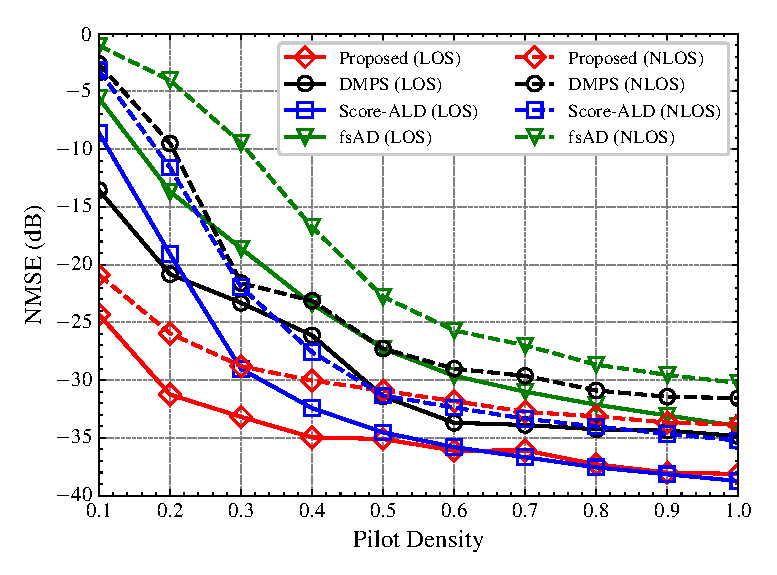
\includegraphics[width=0.48\textwidth]{images/20251013/fig_1.eps}
\caption{Impact of pilot density on the NMSE performance at SNR of 30dB for LOS and NLOS channels.}
\label{fig_sim_1}
\end{figure}

\begin{figure}[!t]
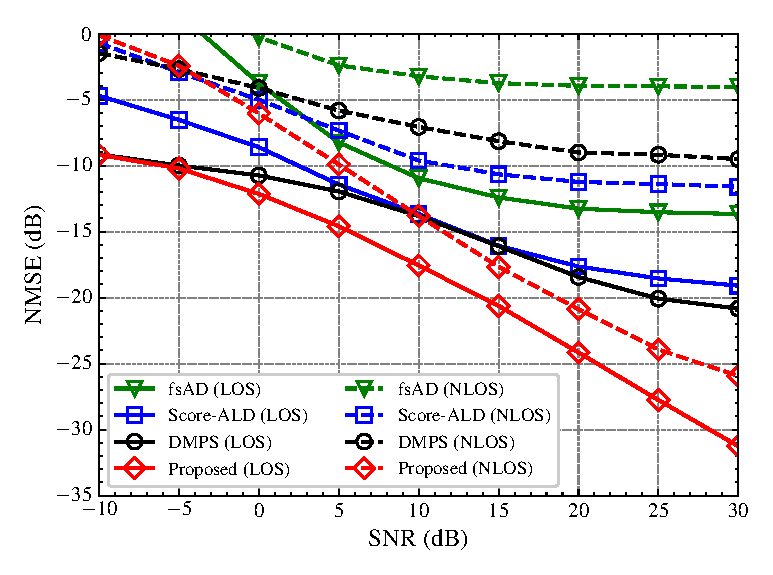
\includegraphics[width=0.48\textwidth]{images/20251013/fig_2.eps}
\caption{Channel estimation performance in terms of NMSE with pilot density of 0.2 for LOS and NLOS channels.}
\label{fig_sim_2}
\end{figure}

\tred{
Fig.~\ref{fig_sim_2} presents the NMSE performance versus SNR
at a fixed pilot density of $\rho$=0.6 to evaluate estimation fidelity.
The fsAD baseline shows a distinct error floor around -14 dB,
which is attributable to model mismatch. Its fixed sparsity assumption deviates from the true channel structure.
This limits performance once thermal noise is no longer the dominant error source. While all DM-based methods overcome this model mismatch, they exhibit their own error floors. DMPS and Score-ALD show floors around -21 dB and -19 dB, respectively. This is due to algorithmic approximation errors in their posterior score modeling. In sharp contrast, our proposed method maintains a linear performance improvement. It achieves an NMSE below -30 dB with increasing SNR, showing no error floor. This demonstrates that our moment matching-based approach is highly effective. By rigorously incorporating the local posterior covariance, it minimizes error accumulation. This eliminates the approximation-induced error floor that plagues other advanced estimators.
}

\tred{
Table~\ref{tab:table1} summarizes the computational efficiency of the proposed method. A superior trade-off between estimation accuracy and latency is demonstrated. Notably, the proposed method is approximately 65 times faster than Score-ALD. This latency reduction stems from requiring significantly fewer neural function evaluations (NFEs). This is in contrast to Score-ALD's iterative annealed Langevin dynamics. While our method has a slightly higher per-step complexity than DMPS, this deliberate trade-off is highly effective. The added computation is for rigorously estimating the local posterior covariance. This is achieved using Tweedie's formula as part of our moment matching approach. This targeted increase in complexity is precisely what enables our method to eliminate the performance-limiting error floors observed in baseline methods, as shown in Fig.~\ref{fig_sim_2}. Consequently, our approach offers a compelling balance, delivering state-of-the-art accuracy without prohibitive latency.
}

\begin{table}[!t]
\centering
\renewcommand{\arraystretch}{1.1} 
\caption{Computational complexity \\for DM-based channel estimation methods}
\label{tab:table1}
\begin{tabular}{M{0.20\columnwidth}|M{0.21\columnwidth}|M{0.20\columnwidth}|M{0.20\columnwidth}}
\hline
\textbf{Method} & \textbf{FLOPs} & \textbf{NFEs} & \textbf{Latency (s)} \\
\hline
Proposed & \(4.899 \times 10^9\) & 20 & 1.29 \\
\hline
Score-ALD\cite{arvinteMIMOChannelEstimation2023} & \(1.028 \times 10^{12}\) & 6933 & 84.97 \\
\hline
DMPS\cite{zhouGenerativeDiffusionModels2025} & \(3.184 \times 10^{10}\) & 130 & 1.27 \\
\hline
\end{tabular}
\end{table}

\section{Conclusions}

\tred{
In this letter, a novel channel estimation method has been proposed for massive MIMO systems. The method effectively addresses estimation accuracy, pilot overhead, and complexity. Our approach performs accurate and efficient diffusion posterior sampling. It incorporates posterior covariance based on the moment matching principle and Tweedie's formula. This proved crucial for overcoming the performance cliff observed in pilot-scarce regimes. From the simulation results, it was demonstrated that the proposed method achieves superior estimation accuracy compared to state-of-the-art baselines. This advantage is especially pronounced under severe pilot scarcity. Furthermore, it eliminates the error floor present in other advanced estimators at high SNRs. These gains are achieved while maintaining a comparable computational complexity. In future work, the extension of the proposed method to wideband and multi-user scenarios can be explored.
}
\bibliographystyle{IEEEtran}
% \bibliography{bib/IEEEabrv,bib/references}
\bibliography{bib/references}
\end{document}

